\subsection{GuestCreator}
\label{sub:GuestCreator}

GuestCreatormodulet har til opgave at oprette en ny gæst i databasen når brugeren er en gæst der ønsker adgang til systemet.

\subsubsection{Funktionalitet}
\label{ssub:GuestCreator_funktionalitet}
GuestCreatoren popper op når man i loginmodulet ønsker at oprette en ny gæst. Brugeren indtaster dernæst information omkring sig selv, båden samt udrejse dato. Dernæst bliver gæsten gemt i databasen.

\begin{figure}
  \centering
  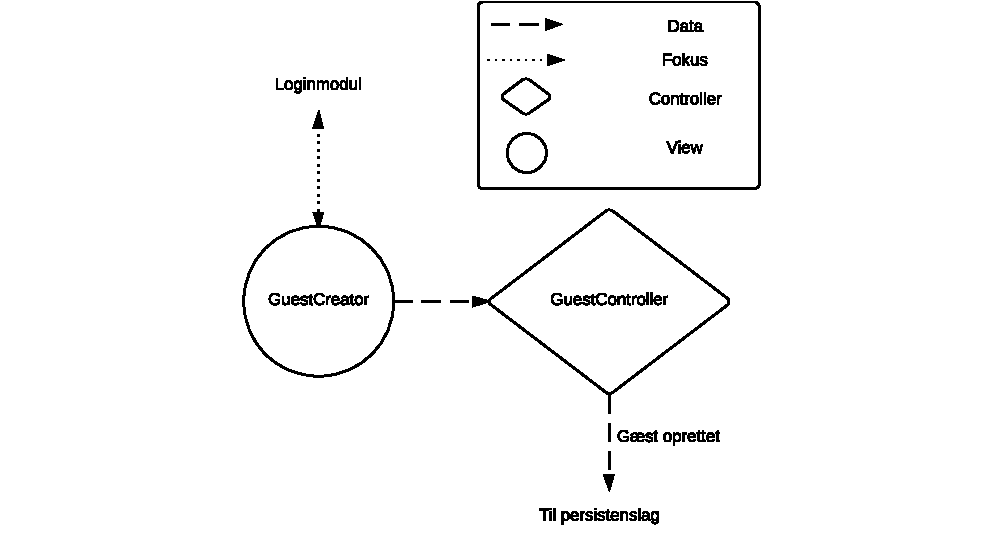
\includegraphics[width=\textwidth]{newguest-diagram.pdf}
  \caption{GuestCreator diagram}
  \label{fig:guestcreator}
\end{figure}

\subsubsection{Implementation}
\label{ssub:GuestCreator_implementation}

GuestCreatormodulet består af et GuestCreator-element og en GuestController. Det indtastede data fra brugeren i GuestCreator-elementet sendes videre til GuestControlleren, som kommunikere med persistenslaget der derefter gemmer informationen om den nye gæst. 